\chapter{Apprendimento automatico}\label{chap:AI_ML}
In questo capitolo si introducono i principali problemi e le principali tecniche risolutive nel campo dell'apprendimento automatico.
Nel~\Cref{sec:imparare_dai_dati} si definisce il termine apprendimento automatico; nel~\Cref{sec:tipi_problemi_ml} si categorizzano i principali problemi di apprendimento automatico; nel~\Cref{sec:comuni_approcci_risolutivi} si descrivono i più comuni approcci risolutivi; nel~\Cref{sec:bias_variance_tradeoff} si introduce la problematica dell'\emph{overfitting}/\emph{underfitting}; nel~\Cref{sec:valutazione_modelli} si descrivono le principali metriche di valutazione dei modelli di apprendimento automatico; nel~\Cref{sec:model_selection} si descrivono infine le principali tecniche per selezionare i migliori iperparametri per addestrare un modello su un certo dataset.

\section{Imparare dai dati}\label{sec:imparare_dai_dati}
Risolvere un problema utilizzando un computer richiede un algoritmo, una sequenza di passi da poter implementare ed eseguire. 
Per alcuni problemi sono noti uno o più algoritmi in grado di trovare soluzioni: ordinare una sequenza di numeri, per esempio, è un compito per cui sono noti diversi algoritmi. 
Per alcuni problemi, invece, è possibile identificare i dati in input, i dati in output, ma non si conosce la procedura per trasformare da input ad output. 
Quali sono i passi per considerare un'\textit{e-mail} come posta indesiderata? 
In caso esistano, sono passi applicabili per ogni casella di posta elettronica? 
Questi criteri cambiano nel tempo o restano fissi? 
Per un essere umano identificare un messaggio come indesiderato è relativamente facile; per una macchina no.

Il fatto che non si possano formalizzare manualmente le caratteristiche che rendono una \emph{e-mail} indesiderata (o che si possa ma sia sconveniente farlo), non vuol dire che queste caratteristiche non esistano. 
Ci sono, ma sono ``nascoste'' tra i dati.
L'apprendimento automatico è una branca dell'intelligenza artificiale che studia tutti quei sistemi in grado di apprendere autonomamente analizzando insiemi (più o meno grandi) di dati, per poi eseguire delle predizioni accurate su dati mai visti prima. 
Oltre alla caratteristica di risolvere compiti che richiedono intelligenza, le tecniche di apprendimento automatico possono prevedere il loro continuo miglioramento, adattando i modelli nel tempo.
Per esempio, i sistemi in grado di identificare posta indesiderata possono essere aggiornati nel tempo con l'aggiunta di nuovi esempi di messaggi segnalati dall'utente come indesiderati.

Lo studio dei modelli di apprendimento automatico si concentra su due compiti principali: definire procedure di addestramento e definire procedure di inferenza. 
In genere l'obiettivo principale è quello di costruire dei modelli efficaci in grado di eseguire predizioni affidabili secondo delle metriche definite in base al problema trattato. 
In altri scenari, caratterizzati da una scarsità di risorse sia computazionali che temporali, è invece necessario enfatizzare l'efficienza del modello in fase di predizione, idealmente senza sacrificare buone capacità di inferenza.

\section{Categorizzazione dei problemi di apprendimento automatico}\label{sec:tipi_problemi_ml}
Ipotizziamo che esista la funzione $f:\mathcal{X}\rightarrow\mathcal{Y}$ ignota. 
Un algoritmo di apprendimento automatico costruirà un modello $\hat{f}:\mathcal{X}\rightarrow\mathcal{Y}$ che approssima $f$ a partire da un insieme di dati di addestramento $\mathcal{S}=\{(x_i, y_i)\}$, dove $\mathcal{S} \subset \mathcal{X} \times \mathcal{Y}$.
L'insieme $\mathcal{X}$ indica i possibili input del modello. Semplificando, si può pensare a $\mathcal{X} \in \mathbb{R}^d$, quindi ogni dato in input è un vettore $\Vec{x}_i=[x_i^1,\dots,x_i^d]$.
Ogni componente dei vettori di input è chiamata attributo (in inglese \emph{feature}).
I dati $y_i \in \mathcal{Y}$ sono chiamati \emph{etichette}; si indicano invece le predizioni di un modello come $\hat{y} = \hat{f}(\Vec{x})$. 

Si parla di apprendimento supervisionato quando l'algoritmo di apprendimento richiede la presenza delle etichette $y_i$ in fase di addestramento; si parla di apprendimento non supervisionato in caso contrario.
Si menziona per completezza l'esistenza di una terza categoria, l'apprendimento per rinforzo, che include algoritmi che cercano di costruire degli ``agenti intelligenti'' che identificano la miglior sequenza di operazioni seguendo dei meccanismi di ricompensa e penalizzazione. 
Gli agenti stessi possono avere un effetto nel ``mondo'' in cui stanno operando, modificando la scelta delle operazioni da compiere.

Un altra possibile suddivisione dei problemi di addestramento automatico è quella in problemi di classificazione e problemi di regressione.
Per un problema di regressione le etichette $y$ assumono valori continui, mentre per un problema di classificazione le etichette $y$ assumono valori discreti. 
Predire il prezzo di vendita di un immobile a partire dalle alcune sue caratteristiche è, per esempio, un problema di regressione, perché il prezzo di vendita è un valore continuo;
identificare se un immagine contiene un gatto oppure no è invece un problema di classificazione, perché la predizione è un valore discreto uguale a ``vero'' oppure ``falso''.

I problemi di classificazione sono a loro volta ulteriormente suddivisi in base alla forma delle etichette. Si identificano:
\begin{itemize}
    \item Problemi di classificazione binaria: la predizione è una sola etichetta tra due possibili etichette, per esempio $\hat{y} \in \{0,1\}$. A prescindere dal valore numerico utilizzato, le due possibili classi son chiamate classe positiva e classe negativa.
    \item Problemi di classificazione multi-classe: la predizione è un vettore di $k$ componenti, ognuno ad indicare una possibile classe. Tra tutte le possibili classi, una predizione ne identifica solo una come positiva. Scegliendo $\hat{y}^i \in \{0,1\}$ con $i=1,\dots,k$, una predizione valida soddisferà l'equazione $\sum_{j=1}^{k} \hat{y}^j =1$.  
    \item Problemi di classificazione multi-etichetta: come problemi di classificazione multi-classe, con la differenza che più di un etichetta può essere predetta come positiva. Le classi non sono mutualmente esclusive. Scegliendo $\hat{y}^i \in \{0,1\}$ con $i=1,\dots,k$, una predizione valida soddisferà l'equazione $\sum_{j=1}^{k} \hat{y}^j \geq 1$.  
\end{itemize}

Anche per problemi di regressione, in caso i valori da predire siano più di uno, si parla di regressione multi-target.

I principali problemi di apprendimento non supervisionato sono invece:
\begin{itemize}
    \item \emph{Clustering}: lo scopo è quello di suddividere un insieme di dati non etichettati in sottoinsiemi più piccoli sulla base di criteri di similarità o distanza geometrica.
    \item Riduzione della dimensionalità: lo scopo è quello di trasformare i dati originali in uno spazio con meno dimensioni senza perdita significativa di informazione.
    \item Regole di associazione: lo scopo è quello di estrarre dai dati delle relazioni significative nella forma di implicazione ``se $x$ allora $y$''.
\end{itemize}

Ricapitolando, l'obiettivo di una procedura di addestramento automatico è quello di approssimare $f$ con $\hat{f}$ in modo accettabile.
La valutazione della bontà di un modello è una parte fondamentale del processo.
In base al tipo di problema, al tipo di dati, all'ambito reale di applicazione del modello, si utilizzano metriche e tecniche diverse.
Questi aspetti saranno approfonditi nei~\Cref{sec:valutazione_modelli,sec:model_selection}.


\section{Comuni approcci risolutivi}\label{sec:comuni_approcci_risolutivi}
In questa sezione si descrivono brevemente alcuni comuni algoritmi per risolvere i problemi tipici dell'apprendimento automatico categorizzati nel~\Cref{sec:tipi_problemi_ml}.
I modelli \emph{support vector machine} saranno invece descritti in dettaglio nel~\Cref{chap:SVC}.

\subsection{K-Nearest Neighbors}\label{sec:ml:knn}
\emph{K-Nearest Neighbors} (KNN), descritto in dettaglio in~\cite{KNN}, è un algoritmo di apprendimento automatico che può essere utilizzato sia per problemi di classificazione che  per problemi di regressione. 
L'idea alla base del funzionamento è quella di predire un etichetta (continua o discreta) basandosi su una misura di vicinanza per i punti dell'insieme di addestramento. 
Secondo questa caratteristica, così come i modelli \emph{support vector machine} che si vedranno in seguito, anche KNN è un \emph{instance based learner}, ovvero un modello definito da un sottoinsieme di dati di addestramento, utilizzati per fare predizioni su nuovi dati.

Per problemi di classificazione binaria e multi-classe, KNN individua i K punti dati più vicini a un punto sconosciuto $\Vec{x}_\text{new}$. 
La classe più comune tra i K vicini diventa la classe prevista per il punto $\Vec{x}_\text{new}$. 
In~\Cref{fig:knn_example} si mostra un esempio di classificazione con $K=3$.
\begin{figure}
    \centering
    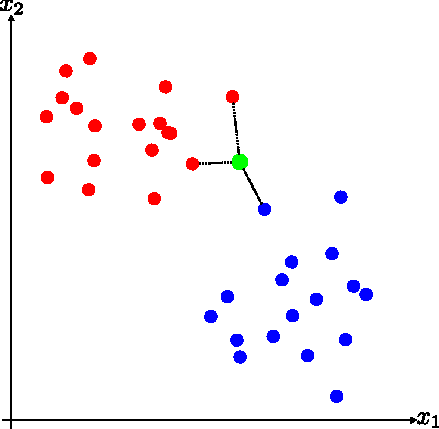
\includegraphics[width=0.7\linewidth]{img/KNN.pdf}
    \caption{Esempio di applicazione della regola di classificazione KNN con $K=3$. I colori blu e rosso identificano le due possibili classi. Il punto color verde è il punto per cui predire la classe.
    Il nuovo punto sarà etichettato rosso perché la maggioranza dei punti vicini (raggiunti dai segmenti tratteggiati) appartiene a quella classe.}
    \label{fig:knn_example}
\end{figure}

Per problemi di regressione, invece, si calcola la predizione per un punto $\Vec{x}_\text{new}$ come media dei valori dei K punti vicini.

L'utilizzo di un modello KNN richiede la scelta dell'iperparametro $K$.
Un $K$ troppo piccolo porterà a previsioni instabili, mentre un $K$ troppo grande porterà a previsioni troppo generalizzate. 
Come per altri modelli si rende in genere necessaria una fase di \emph{model selection} (~\Cref{sec:model_selection}) per identificare i migliori iperparametri. 
In aggiunta a definire $K$ è necessario definire una misura della distanza tra punti.

KNN è un algoritmo facile da comprendere e implementare, ma ha delle evidenti limitazioni. 
\`E sensibile alla scelta di K ed è particolarmente inadatto per dataset di grandi dimensioni a causa dello spazio richiesto (tutti i dati di addestramento) ma soprattutto per il costo computazionale, dato che è necessario calcolare la distanza rispetto ad ogni elemento per ogni predizione, anche se nella pratica si possono utilizzare strutture dati o algoritmi di ricerca più efficienti.

Nonostante queste limitazioni KNN rimane una scelta valida da utilizzare con dataset di piccole dimensioni.

\subsection{Alberi decisionali}
Gli alberi decisionali, descritti in dettaglio in~\cite{decision_tree}, sono modelli che effettuano predizioni basandosi su una struttura dati ad albero creata durante il processo di addestramento. Ogni nodo interno rappresenta una regola, che valutata su un nuovo dato $\Vec{x}_\text{new}$, indicherà in quale sotto-albero procedere con la predizione, fino ad arrivare ad una foglia che identifica la classe da assegnare. Il processo di addestramento di un albero decisionale identifica quali sono le regole più vantaggiose da utilizzare per raggiungere buone performance di classificazione. 
L'algoritmo di addestramento più noto è CART. 
La bontà di ogni decisione, o in altre parole il criterio con cui creare i nodi interni dell'albero, viene valutata secondo una metrica, tra le più famose: \emph{Gini impurity}, \emph{information gain} e \emph{root mean squared error (RMSE)}. 
\begin{figure}
    \centering
    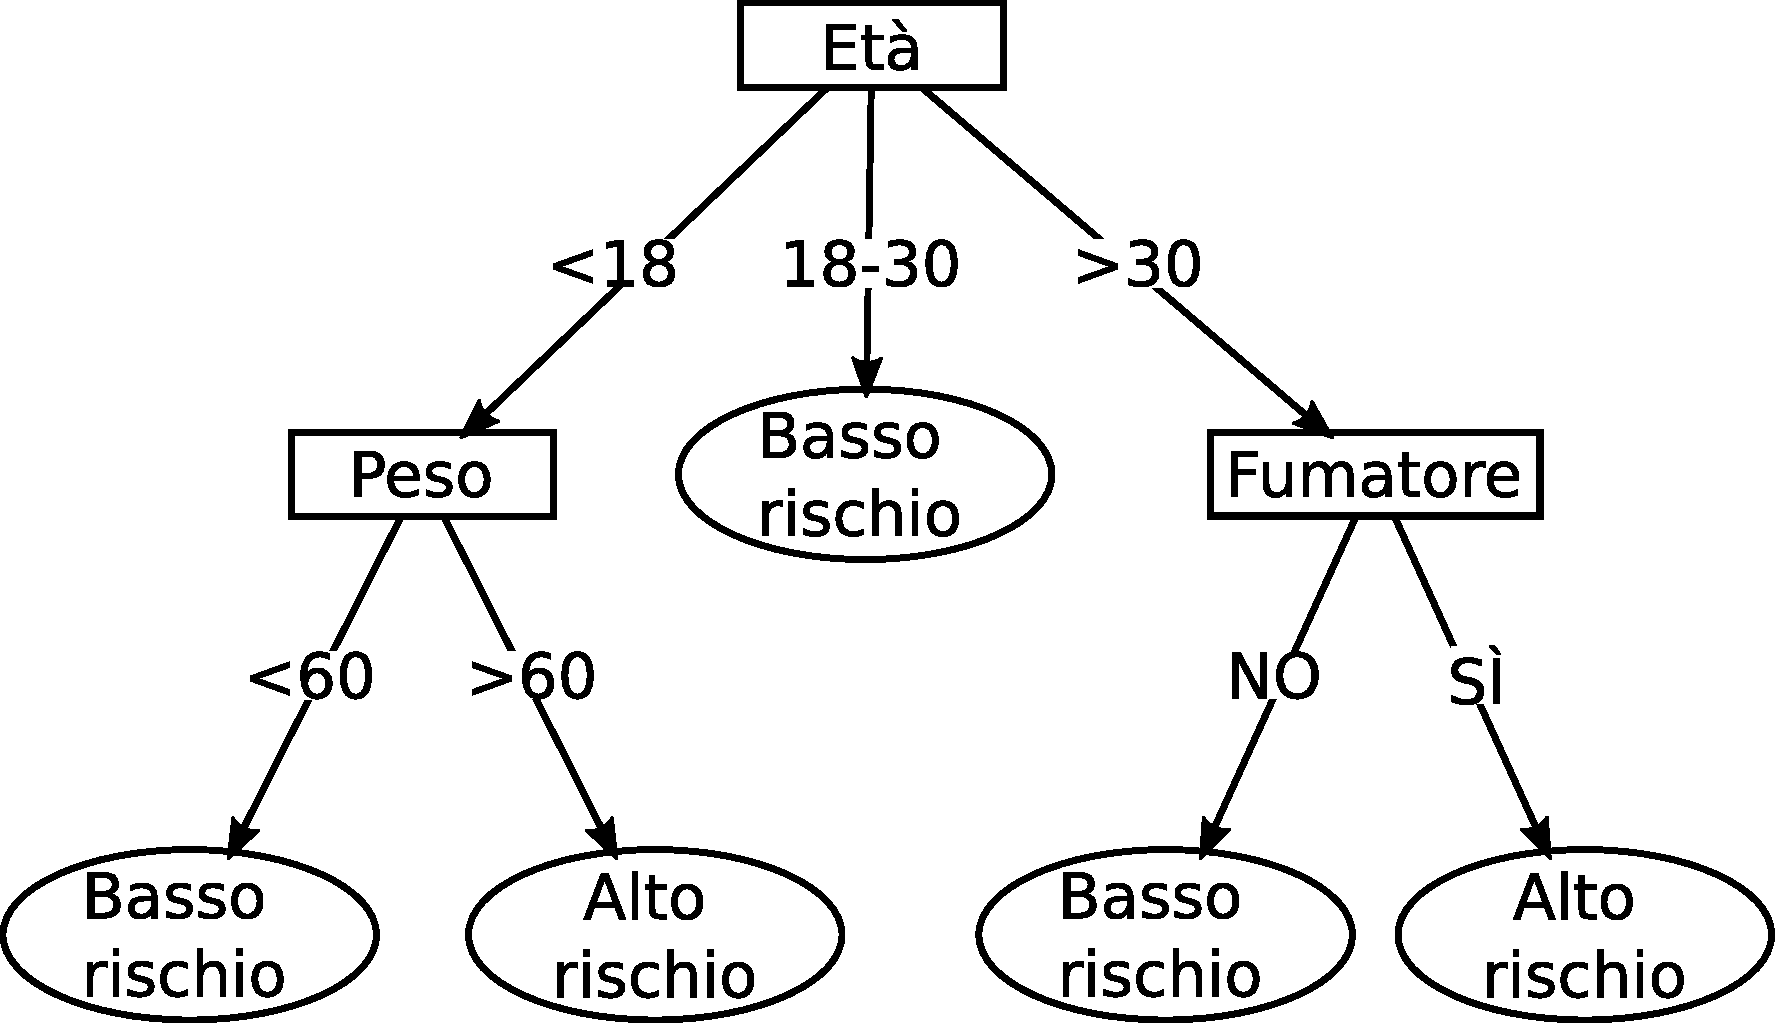
\includegraphics[width=0.7\linewidth]{img/decision_tree.pdf}
    \caption{Esempio semplificato di un possibile albero di decisione per il rischio di malattia cardiaca. I nodi rettangolari identificano delle regole, in questo caso un semplice controllo sull'attributo con il nome del nodo. I nodi foglia ovali identificano il valore della predizione.}
    \label{fig:decision_tree}
\end{figure}
Gli alberi decisionali sono modelli semplici e hanno il pregio di essere modelli \emph{white box}, ovvero sono noti i criteri per cui è eseguita una predizione.
Hanno però la tendenza a fare \emph{overfitting}, dato che è sempre possibile ottenere un albero con una foglia per ogni dato di addestramento, e soffrono di \emph{variance error}, dato che anche minimi cambiamenti nell'insieme di addestramento potrebbero avere un influenza enorme sul modello prodotto.
Queste problematiche saranno meglio discusse nel~\Cref{sec:bias_variance_tradeoff}.
Per queste limitazioni, nella pratica sono molto più utilizzate le \emph{ensemble} di alberi decisionali, utilizzando tecniche come \emph{bagging} e \emph{boosting}.
Un modello \emph{ensemble} è composto da molteplici modelli ``interni'' combinati per ottenere prestazioni migliori; non necessariamente i modelli sono omogenei.

\subsubsection{Random Forest}
Un primo metodo per creare un \emph{ensemble} di alberi decisionali è chiamato \emph{bagging predictors} (introdotto in~\cite{bagging_predictors}), termine che deriva da \emph{\textbf{b}ootstrap} \emph{\textbf{agg}regat\textbf{ing}}.
L'idea alla base del funzionamento è la seguente: il dataset di addestramento originale $D$ viene utilizzato per creare $k$ ulteriori dataset di dimensioni minori (circa $\frac{2}{3}$ del dataset originale) contenenti elementi estratti da $D$ uniformemente a caso con ripetizione.
Su questi $k$ dataset si addestrano (singolarmente) altrettanti alberi di decisione, per poi creare un modello unico che aggrega le loro predizioni utilizzando una regola sensata per il problema trattato: per un problema di classificazione, per esempio, si potrebbe utilizzare un voto di maggioranza.

I modelli \emph{random forest}, introdotti in~\cite{random_forest}, estendono l'approccio \emph{bagging} introducendo anche la randomizzazione degli attributi. 
Ognuno dei $k$ modelli interni sarà addestrato su un sottoinsieme  di attributi selezionati casualmente senza ripetizione, una sola volta per l'intero albero oppure ad ogni creazione di un nodo interno.
Le predizioni sono poi aggregate come nei \emph{bagging predictors}.

\begin{figure}
    \centering
    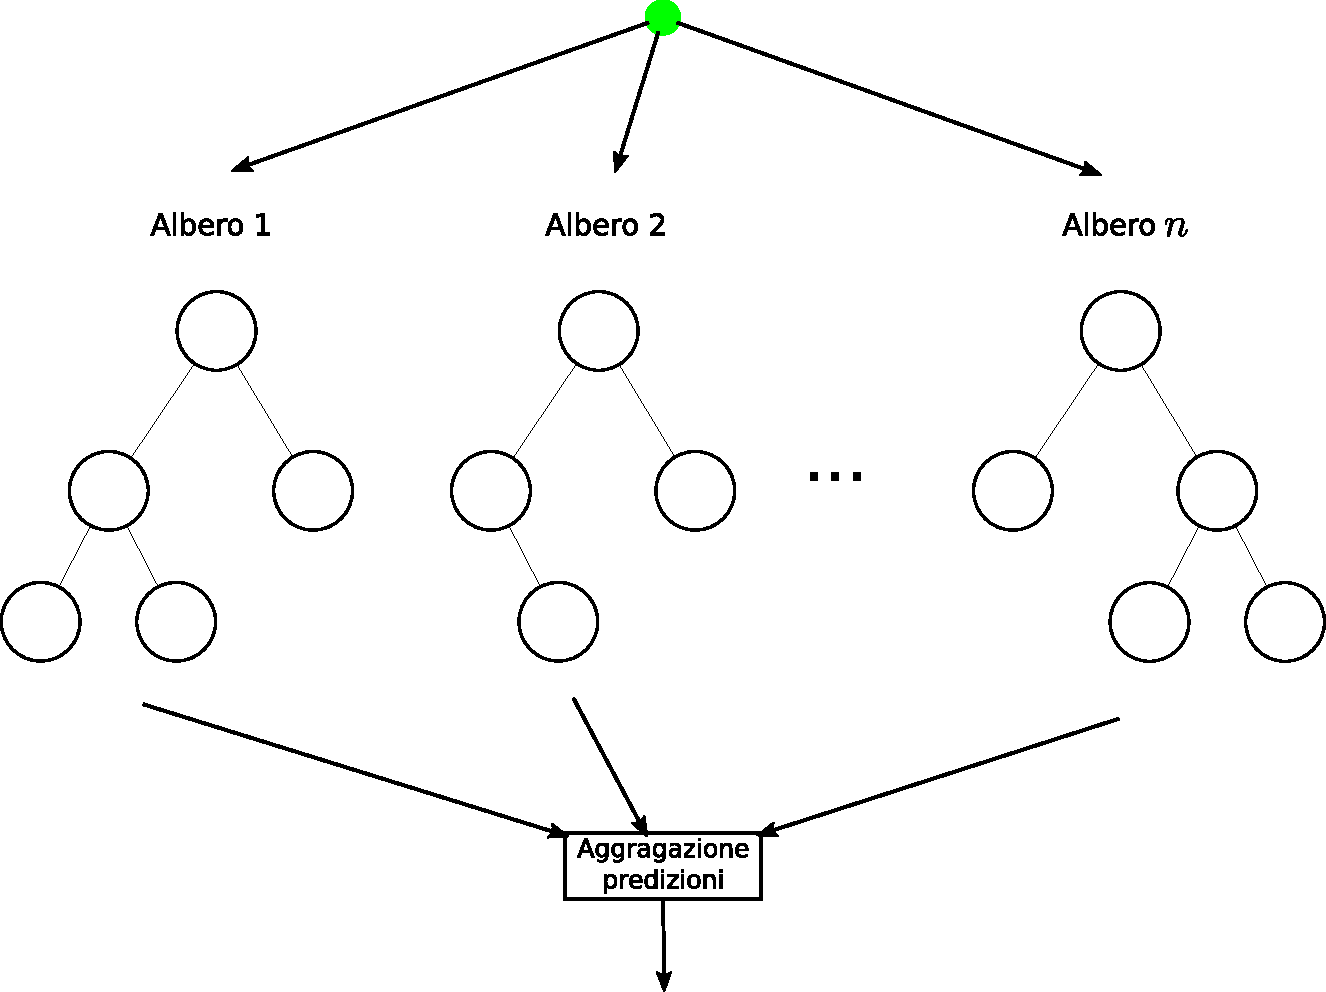
\includegraphics[width=0.7\linewidth]{img/random_forest.pdf}
    \caption{Esempio di \emph{random forest}. Il modello è composto da un insieme di alberi interni, ognuno addestrato su un diverso sottoinsieme di dati e di attributi. Un nuovo esempio da classificare, in questa figura il punto verde, viene classificato da ogni sotto-albero singolarmente, per poi produrre una predizione singola utilizzando una regola di aggregazione delle predizioni interne.}
    \label{fig:random_forest}
\end{figure}

\subsubsection{Boosting}
Un altro approccio per creare \emph{ensamble} di alberi è quello che sfrutta la tecnica chiamata \emph{boosting}, che consiste nel combinare molteplici \emph{waeak learner} (in questo caso alberi decisionali molto semplici, anche un solo nodo interno) in modo da ottenere, combinandoli tra loro, uno \emph{strong learner}, ovvero un modello in grado di trattare problemi complessi.
Relativamente agli alberi di decisione gli approcci più famosi sono \emph{AdaBoost}~\cite{adaboost} e \emph{XGboost}~\cite{xgboost}

%\subsection{Logistic regression}

\subsection{Reti neurali}

Le reti neurali, descritte in dettaglio in~\cite{neural_networks}, sono un tipo di modello di apprendimento automatico ispirato alla struttura del cervello umano, composto da neuroni collegati tra di loro e in grado di scambiare impulsi.
Nella categoria reti neurali rientra una quantità di modelli molto ampia e varia.

Le reti neurali nascono come estensione del modello \emph{perceptron}~\cite{1958_perceptron}; viene riportato un esempio in~\Cref{fig:perceptron}.
Un \emph{perceptron} è un modello molto semplice composto da un singolo neurone artificiale.
Il neurone riceve in ingresso un vettore $\Vec{x}=\{x_1,\dots,x_n\}$ con $x_i \in \mathbb{R}$ ed emette un output 
\begin{equation*}
    \hat{y} = \theta\left(\sum_{i=1}^{n}x_iw_i +b\right),
\end{equation*} 
dove $w_1,\dots,w_n \in \mathbb{R}$ sono chiamati pesi, $b \in \mathbb{R}$ è il \emph{bias} e $\theta$ è la \emph{funzione di attivazione}, che nel perceptron originale è la \emph{step function} 
\begin{equation*}
    \sigma(x) =
    \begin{cases*}
      1 & se $x>0$, \\
      0 & se $x\leq0$.
    \end{cases*}
\end{equation*}
\begin{figure}
    \centering
    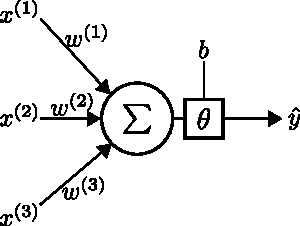
\includegraphics[width=0.5\linewidth]{img/perceptron.pdf}
    \caption{Esempio di \emph{perceptron}. Le $x_1,x_2,x_3$ identificano gli input, mentre $\hat{y}$ l'output del modello. I parametri $w_1,w_2,w_3$ sono i pesi mentre $b$ è l'opzionale \emph{bias}. $\theta$ è la funzione di attivazione.}
    \label{fig:perceptron}
\end{figure}
Il perceptron è un modello semplice ma è la base per la creazione delle reti neurali.
Una rete neurale è composta da molteplici \emph{perceptron} collegati tra loro, organizzati in più strati: strato di \emph{input}, strati nascosti e strati di \emph{output}.
Le reti neurali con questa struttura sono infatti anche chiamate \emph{multi-layer perceptron}.
A seconda del numero di strati nascosti è possibile suddividere le reti neurali in \emph{shallow} o \emph{deep}.
Si mostra in~\Cref{fig:NN} un esempio di semplice rete neurale. 
\begin{figure}
    \centering
    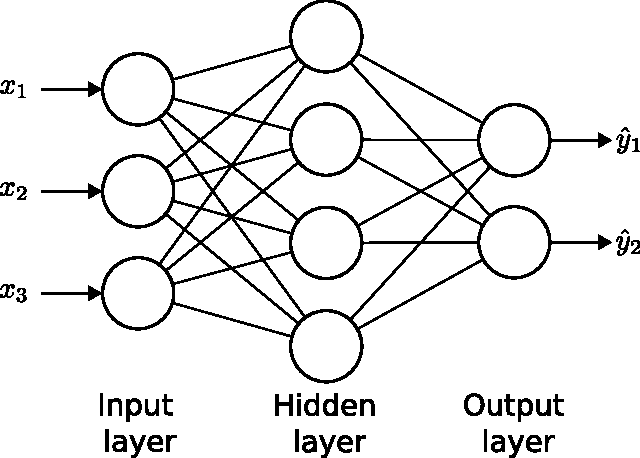
\includegraphics[width=0.5\linewidth]{img/nn.pdf}
    \caption{Esempio di una semplice rete neurale con 3 neuroni di input e 2 di output.}
    \label{fig:NN}
\end{figure}
Le reti neurali descritte fino ad ora sono chiamate \emph{feed-forward} perché i dati di addestramento fluiscono dallo strato di \emph{input} fino a quello di \emph{output}. 
Esistono altre tipologie di reti con strutture più complesse, per esempio le reti ricorrenti, le reti convoluzionali, le reti generative e altre numerose varianti e combinazioni.

L'addestramento di una rete neurale \emph{feed-forward} è effettuato con l'algoritmo di retro-propagazione dell'errore:
in seguito alla fase \emph{forward-pass} in cui i dati passano nella rete fino a produrre la predizione, si calcola l'errore; percorrendo poi a ritroso la rete nella \emph{backwards-pass} si aggiustano i pesi e i \emph{bias} dei neuroni in modo da ridurre l'errore misurato.
L'algoritmo procede iterativamente.
In base alla tipologia di rete neurale esistono diversi algoritmi di addestramento, ma in generale si utilizza un metodo del gradiente per ridurre iterativamente l'errore sui dati di addestramento.

\section{Valutazione dei modelli}\label{sec:valutazione_modelli}
Nel campo dell'apprendimento automatico è di fondamentale importanza utilizzare delle metriche per misurare l'efficacia dei modelli sia durante la fase di addestramento che durante la fase di utilizzo su dati mai visti.
A prescindere dalla metrica utilizzata, la bontà di un modello è in genere misurata su un \emph{test set}, ovvero un sottoinsieme dei dati disponibili utilizzato solo ed esclusivamente per questo scopo.
L'insieme di \emph{test} simula un insieme di dati nuovi mai visti dal modello.
Per una valutazione significativa è necessario un \emph{test set} significativo, composto da un numero sufficiente di elementi e con una distribuzione di etichette il più fedele possibile ad uno scenario reale.
% L'errore principale da evitare nella valutazione di un modello è il così detto \emph{data leakage}. 
% Questo termine identifica tutte quelle situazioni in cui delle caratteristiche che dovrebbero essere ignote al modello in fase di addestramento vengono invece erroneamente inserite nel set di addestramento.
% Consideriamo per esempio un problema di regressione in cui si vuole predire il valore dello stipendio annuo di alcuni lavoratori a partire da un dataset di caratteristiche rilevanti: se una di queste caratteristiche fosse il valore di stipendio mensile, avremmo una situazione di \emph{data leakage}, perché il dato da predire è sostanzialmente utilizzato dal modello come input.
Generalmente, si divide l'insieme di dati disponibile in due parti: un \emph{train set} utilizzato per l'addestramento ed un \emph{test set} utilizzato esclusivamente per la valutazione. 
La scelta della composizione del \emph{test set}, come accennato prima, è critica, esattamente come la scelta della composizione del \emph{train set}.
Ipotizzando di avere a disposizione un \emph{test set} di qualità, ci sono altri criteri che guidano la valutazione di un modello.

La quantità di dati disponibili è un fattore che influisce anche sulla tipologia di modello utilizzabile.
Alcuni modelli richiedono grandi quantità di dati per essere addestrati, mentre invece altri modelli sono più adatti per piccoli dataset. 

Il tipo di modello utilizzato ed il tipo di problema trattato guida la scelta di una metrica adatta: per problemi di classificazione, ad esempio, ha senso utilizzare il numero di predizioni corrette in rapporto al numero di predizioni totali; per problemi di regressione, invece, non è possibile utilizzare lo stesso criterio perché le predizioni son valori continui e non è semplicemente possibile contare il numero di predizioni corrette. 

\subsection{Metriche per modelli di classificazione}\label{sec:metriche_valutazione_modelli}
Considerando per semplicità un problema di classificazione binaria, si definiscono:
\begin{itemize}
    \item \textbf{TP} il numero di predizioni correttamente identificate nella classe positiva.
    \item \textbf{TN} il numero di predizioni correttamente identificate nella classe negativa.
    \item \textbf{FP} il numero di predizioni erroneamente identificate nella classe positiva.
    \item \textbf{FN} il numero di predizioni erroneamente identificate nella classe negativa.
\end{itemize}
Queste quantità sono spesso organizzate in una matrice, chiamata matrice di confusione.
Viene riportato in~\Cref{tab:matrice_confusione} un esempio di matrice di confusione per un classificatore binario immaginario che identifica o meno la presenza di una malattia a partire da un referto preso in input.
\begin{table}[h]
    \centering
    \begin{tabular}{l|l|c|c|}
        \multicolumn{2}{c}{}&\multicolumn{2}{c}{Effettive}\\
        \cline{3-4}
        \multicolumn{2}{c|}{} & Positive & Negative\\
        \cline{2-4}
        \multirow{2}{*}{Predizioni}& Positive & 1 (TP) & 1 (FP) \\
        \cline{2-4}
        & Negative & 8 (FN) & 90 (TN) \\
        \cline{2-4}
    \end{tabular}
    \caption{Esempio di matrice di confusione, da \protect\footnotemark.}
    \label{tab:matrice_confusione}
\end{table}

\footnotetext{\url{https://developers.google.com/machine-learning/crash-course/classification/accuracy?hl=en}}

\subsubsection{Accuratezza} La metrica accuratezza è una delle metriche principali utilizzate per problemi di classificazione, ed è calcolata come:
\begin{equation*}
    \textrm{\emph{Accuratezza}} = \frac{\text{Numero di predizioni corrette}}{\text{Numero di predizioni totali}} = \frac{\text{TP} + \text{TN}}{\text{TP} + \text{TN} + \text{FP} + \text{FN}}.
\end{equation*}
Questa metrica può dare una prima indicazione delle capacità di un classificatore ma può essere poco significativa a seconda del problema considerato, perché non quantifica la distribuzione delle predizioni corrette né la distribuzione di quelle errate.
Nell'esempio in~\Cref{tab:matrice_confusione} l'accuratezza ha valore $0.91$, il che sembrerebbe indicare un buon classificatore.
Per il problema oggetto dell'esempio però, questo valore è ingannevole, dato che 8 pazienti sarebbero classificati dal modello come in salute quando invece non lo sono: questi 8 errori hanno un costo molto alto nel contesto del problema considerato.
L'accuratezza non è sufficiente per valutare questi dettagli.

\subsubsection{Precisione} La metrica precisione, calcolata come
\begin{equation*}
    \textrm{Precisione} = \frac{\text{TP}}{\text{TP} + \text{FP}},
\end{equation*}
è una misura di quanti degli esempi predetti positivi sono effettivamente positivi.
Un modello che predice correttamente tutti gli esempi positivi avrà un valore di precisione uguale ad $1$.
Nell'esempio in~\Cref{tab:matrice_confusione} il valore di precisione è $0.5$: quando un paziente è segnalato come ammalato, lo è effettivamente nella metà dei casi.

\subsubsection{Sensibilità} La metrica sensibilità, calcolata come 
\begin{equation*}
    \textrm{sensibilità} = \frac{\text{TP}}{\text{TP} + \text{FN}},
\end{equation*}
è una misura di quanti degli effettivi veri positivi sono identificati come tali dal modello.
Nell'esempio in~\Cref{tab:matrice_confusione} il valore di sensibilità è $0.11$: tra tutti gli effettivi pazienti ammalati, il modello ne identifica correttamente l'$11\%$.


\subsubsection{F1} La metrica F1, calcolata come 
\begin{equation*}
    \textrm{\emph{F1}} = \frac{2(\text{Precisione} \times \text{sensibilità})}{\text{Precisione} + \text{sensibilità}} = \frac{2\text{TP}}{2\text{TP}+ \text{FP}+ \text{FN}},
\end{equation*}
è una media armonica tra precisione e sensibilità, metriche spesso in contrasto tra di loro. 

\subsection{Metriche per problemi di regressione}
Per dare un'idea di come la valutazione dei modelli di regressione sia diversa rispetto alla valutazione dei modelli di classificazione, si riportano in questo paragrafo alcune comuni metriche per problemi di regressione. 

\subsubsection{Mean squared error (MSE)}
La metrica MSE, calcolata come
\begin{equation*}
    \textrm{MSE} = \frac{1}{n} \sum_{i=1}^{n} (y_i - \hat{y}_i)^2,
\end{equation*}
dove $n$ è il numero di elementi considerati, è la media della differenza tra predizione ed etichetta attuale elevata al quadrato (perché le predizioni possono anche essere valori negativi).

\subsubsection{Root mean squared error (RMSE)}
La metrica RMSE, calcolata come
\begin{equation*}    
    \textrm{RMSE} = \sqrt{\frac{1}{n} \sum_{i=1}^{n} (y_i - \hat{y}_i)^2},
\end{equation*}
dove $n$ è il numero di elementi considerati, non è altro che la radice quadrata della metrica MSE.

\subsubsection{Mean absolute error (MAE)}
La metrica MAE, calcolata come
\begin{equation*}    
    \textrm{MAE} = \frac{1}{n} \sum_{i=1}^{n} |y_i - \hat{y}_i|,
\end{equation*}
dove $n$ è il numero di elementi considerati, diminuisce il peso degli errori gravi rispetto alla metrica MSE.

\subsection{k-fold cross validation}
La procedura $k$\emph{-fold cross validation} è una tecnica per ottenere delle stime robuste di una metrica, valutandola diverse volte su diversi insiemi di \emph{test}.
Il termine $k$ identifica un iperparametro che decide il numero di valutazioni effettuate.
Il funzionamento è il seguente:
\begin{enumerate}
    \item Si suddividono casualmente i dati in $k$ sottoinsiemi, chiamati \emph{fold}.
    \item Per $k$ volte, si sceglie un \emph{fold} da utilizzare come \emph{test} mentre le restanti $k-1$ vengono utilizzate per addestrare un modello. Per ogni iterazione si valuta la metrica sull'insieme di test.
    \item Come stima finale, si calcola la media delle $k$ valutazioni effettuate.
\end{enumerate}
La~\Cref{fig:kfoldcv} mostra graficamente un esempio delle suddivisioni effettuate dal metodo.
\begin{figure}
    \centering
    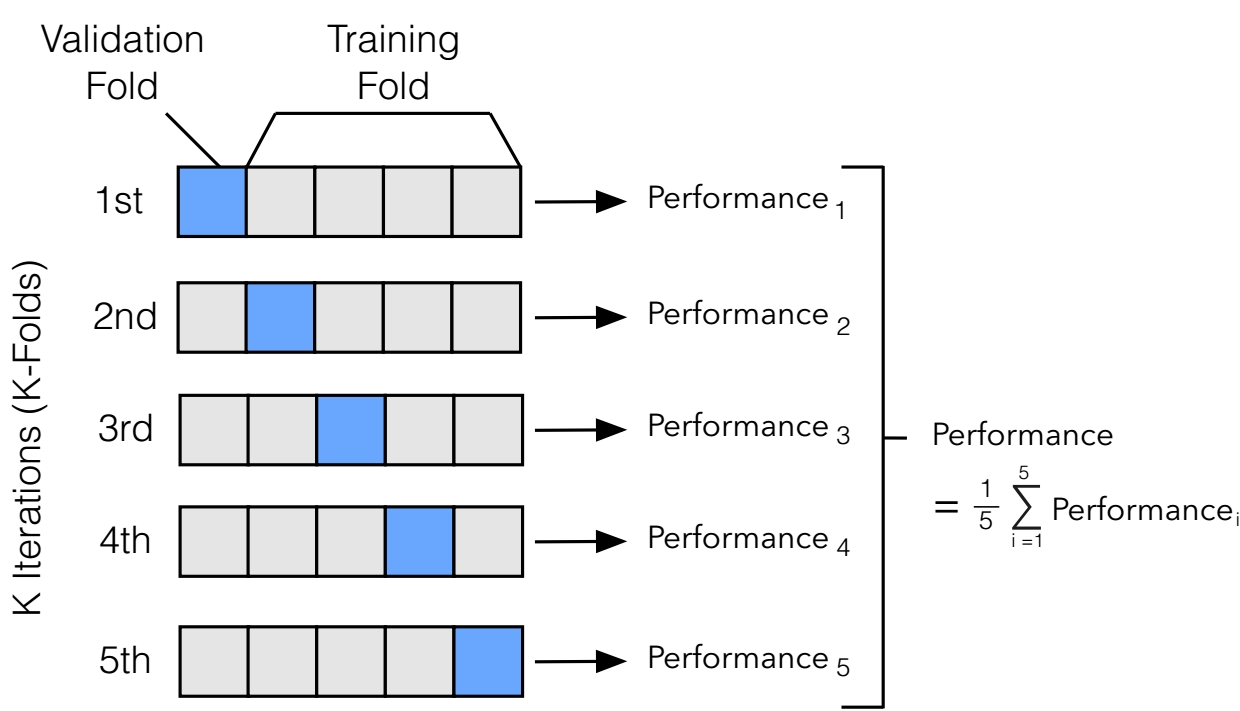
\includegraphics[width=0.7\linewidth]{img/kfoldCV.jpg}
    \caption{Tratto da~\cite{model_evaluation}. Esempio di come \emph{5-fold cross validation} suddivide i dati di addestramento disponibili in 5 parti, utilizzandole tutte una volta come \emph{test}.}
    \label{fig:kfoldcv}
\end{figure}
Si parla di \emph{stratified k-fold cross-validation} quando la procedura mantiene la proporzione delle etichette originali nel creare le diverse suddivisioni.


\section{Selezione dei modelli}\label{sec:model_selection}
L'addestramento di un modello di apprendimento automatico richiede il più delle volte la scelta di un valore per alcuni iperparametri. 
Nel caso dei modelli \emph{k-nearest neighbours} visti nel~\Cref{sec:ml:knn}, per esempio, è necessario fissare un valore per il parametro $k$. 
La scelta di questi eventuali iperparametri è di assoluta importanza, ma non esiste però una regola generica ed automatica per fissare a priori un valore soddisfacente. La scelta dei valori potrebbe dipendere da tanti fattori, come per esempio dalle caratteristiche dei dati a disposizione, oppure dagli obiettivi desiderati (per esempio potrebbe essere preferibile un modello che genera pochissimi falsi negativi a scapito di più falsi positivi).
In genere, si utilizzano dei criteri o degli algoritmi per selezionare le migliori combinazioni di iperparametri per il problema da risolvere: questa fase nel processo di creazione di un modello di addestramento automatico è chiamata \emph{model selection}.
Le tecniche di \emph{model selection} richiedono molteplici esecuzioni dell'algoritmo di addestramento e altrettante valutazioni su un insieme di dati che non può però essere l'insieme di \emph{test}, dato che è riservato per la valutazione finale di un modello. 
L'insieme di \emph{test} simula dei dati mai visti dal modello per stimare la bontà di generalizzazione e non può essere utilizzato per aggiustare gli iperparametri.
In caso lo fosse si verificherebbe lo scenario chiamato come \emph{data leakage}, ovvero l'utilizzo durante l'addestramento di informazioni che non dovrebbero essere usate per non falsare la bontà del modello.
Si descrivono in questo paragrafo le principali tecniche di \emph{model selection}, mentre in~\cite{model_evaluation} si può trovare una descrizione esaustiva.
\subsubsection{Bias pessimistico} Il termine \emph{bias} pessimistico è utilizzato per indicare come la valutazione delle capacità di generalizzazione effettuata su un sottoinsieme dei dati disponibili possa essere troppo pessimistica rispetto alle capacità che si sarebbero potute ottenere addestrando il modello sull'intero insieme di dati.
Purtroppo, utilizzare tutti i dati disponibili durante l'addsestramento renderebbe inaffidabile qualsiasi valutazione effettuata con gli stessi; si preferisce si solito una valutazione pessimistica che una ottimistica.

\subsection{Triplo hold-out}
Si è già discusso di come il dataset di \emph{test} non possa essere utilizzato per aggiustare gli iperparametri di un modello.
Un primo approccio è quello di suddividere in modo leggermente diverso l'insieme totale dei dati a disposizione, prevedendo 3 sottoinsiemi: 
\begin{itemize}
    \item Insieme di addestramento (\emph{test set}): utilizzato per addestrare i modelli.
    \item Insieme di validazione (\emph{validation set}): utilizzato per valutare i modelli con lo scopo di definire i migliori iperparametri.
    \item Insieme di \emph{test} (\emph{test set}): utilizzato in ultima battuta per stimare l'errore di generalizzazione.
\end{itemize}
La selezione di un insieme di validazione è critica tanto quanto la selezione dell'insieme di \emph{test}.

La procedura di selezione del miglior modello procede applicando i seguenti passi:
\begin{enumerate}
    \item si addestrano molteplici modelli con differenti iperparametri utilizzando l'insieme di addestramento;
    \item si valutano le performance di tutti i modelli addestrati utilizzando l'insieme di validazione;
    \item si utilizzano gli iperparametri che hanno generato il modello più performante per addestrare un nuovo modello sull'unione dei dati di addestramento con i dati di validazione, cercando di ridurre il \emph{bias} pessimistico;
    \item si misura la bontà di questo ultimo modello sui dati di \emph{test}.
\end{enumerate}

\subsection{Combinazioni di possibili iperparametri}
I possibili valori per ogni iperparametro sono definiti in una \emph{griglia di iperparametri}.
In base a quali possibili valori vengono provati nella procedura di selezione del miglior modello, si identificano diverse strategie di \emph{grid search} (procedura per provare le varie combinazioni di parametri).

Per ogni approccio possibile, la stima del miglior modello può essere effettuata usando tecniche come \emph{k-fold cross-validation}.

\subsubsection{Grid search}
Il termine è utilizzato per indicare la più semplice delle strategie. Si provano infatti tutte le possibili combinazioni di valori degli iperparametri. 
Questo tipo di strategia è la più esaustiva ma anche la più costosa dal punto di vista computazionale.
Per gli esperimenti descritti nel~\Cref{chap:esperimenti} è stata utilizzata questa tecnica combinata con \emph{5-fold cross-validation} per identificare i migliori parametri.
\subsubsection{Randomized grid search}
Questa strategia seleziona casualmente un sottoinsieme delle possibili combinazioni di iperparametri. 
Il risultato potrebbe variare tra diverse esecuzioni e non c'è la garanzia di trovare la miglior combinazione tra i valori della griglia.
Ciò nonostante questa strategia può comunque fornire un buon risultato e risulta essere una buona opzione nei casi in cui una ricerca esaustiva non sia fattibile. 

\section{Bias-variance tradeoff}\label{sec:bias_variance_tradeoff}
Il termine \emph{bias-variance tradeoff}~\cite{elements-of-statistical-learning} si riferisce ad una caratterizzazione dell'errore di generalizzazione, ovvero la discrepanza tra i valori effettivi e quelli predetti, relativamente ad un insieme di \emph{test} e le relative implicazioni pratiche.

Il concetto può essere formalizzato come in~\cite{elements-of-statistical-learning}, ma ci si limiterà in questo paragrafo a descriverlo sinteticamente con un esempio.
Si ipotizzi di avere disponibile un dataset con le caratteristiche di alcuni pazienti: si pone il compito di costruire un modello per predire se una data persona è a rischio di soffrire di infarto oppure no.
Si consideri ora di costruire un modello molto semplice: un albero di decisione composto da un solo nodo, per cui se l'età del paziente è $>50$ si predice ``rischio alto'' altrimenti ``rischio basso''.
Un modello di questo tipo ha \emph{variance} molto bassa, perché utilizzando anche dati molto diversi da quelli di addestramento, eseguirà predizioni consistenti.
Di contro, questo modello ha \emph{bias} molto alto, perché esegue la predizione solo ed esclusivamente controllando l'età del paziente, evitando di considerare tutte le altre importanti informazioni. 
Il modello non è in grado di approssimare la relazione reale espressa dai dati.
Cambiando approccio, ipotizziamo di addestrare invece un albero di decisione molto profondo, arrivando a generare un nodo foglia per ogni dato di addestramento.
Questo secondo modello avrà \emph{bias} molto basso, perché sarà in grado di classificare correttamente ogni dato di addestramento utilizzando tutte le informazioni disponibili, ma allo stesso tempo avrà \emph{variance} molto alta, perché per dati nuovi faticherà a trovare un percorso radice-foglia adatto.

Un buon modello con buone capacità di generalizzazione deve esibire basso \emph{bias} e bassa \emph{variance}. Si chiama \emph{bias-variance tradeoff} (compromesso appunto) perché è molto difficile minimizzare entrambe queste caratteristiche contemporaneamente. In genere, implementare delle tecniche per migliorare il \emph{bias} fa peggiorare la \emph{variance} e viceversa.
Nonostante ciò, è spesso possibile trovare un modello con buone capacità di generalizzazione. 

Questo problema si traduce nella pratica nel problema di \emph{overfitting} e \emph{underfitting}.
Un modello che soffre di \emph{overfitting} (alta \emph{variance}, basso \emph{bias}) è un modello che si è adattato troppo fedelmente ai dati di addestramento, esibendo pessime performance di generalizzazione. 
Un modello che soffre di \emph{underfitting} (alto \emph{bias}, bassa \emph{variance}) è un modello che non è sufficientemente complesso per modellare le relazioni espresse nei dati ed esibisce pessime performance di generalizzazione.
In~\Cref{fig:esempio_underfitting_overfitting} si visualizza un esempio dei vari scenari \emph{overfitting}, \emph{underfitting} e un esempio di modello con buone capacità di generalizzazione.